% Poncelet's porism: circles with d^2 = R^2 - 2Rr; triangles started anywhere on the outer circle close up.
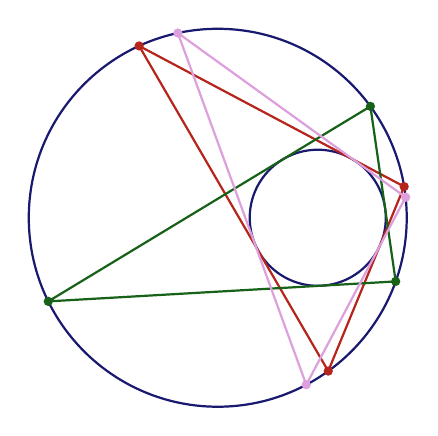
\begin{tikzpicture}[scale=2.4]
\draw[MidnightBlue,thick] (0,0) circle (1.0000);
\draw[MidnightBlue,thick] (0.5292,0.0000) circle (0.3600);
\draw[BrickRed,thick] (-0.4161,0.9093) -- (0.9863,0.1649) -- (0.5846,-0.8113) -- cycle;
\fill[BrickRed] (-0.4161,0.9093) circle (0.7pt) (0.9863,0.1649) circle (0.7pt) (0.5846,-0.8113) circle (0.7pt);
\draw[ForestGreen!70!black,thick] (-0.8968,-0.4425) -- (0.8077,0.5895) -- (0.9415,-0.3369) -- cycle;
\fill[ForestGreen!70!black] (-0.8968,-0.4425) circle (0.7pt) (0.8077,0.5895) circle (0.7pt) (0.9415,-0.3369) circle (0.7pt);
\draw[Plum,thick] (0.4685,-0.8835) -- (-0.2111,0.9775) -- (0.9941,0.1086) -- cycle;
\fill[Plum] (0.4685,-0.8835) circle (0.7pt) (-0.2111,0.9775) circle (0.7pt) (0.9941,0.1086) circle (0.7pt);
\end{tikzpicture}
